\documentclass{beamer}\usepackage[]{graphicx}\usepackage[]{color}
%% maxwidth is the original width if it is less than linewidth
%% otherwise use linewidth (to make sure the graphics do not exceed the margin)
\makeatletter
\def\maxwidth{ %
  \ifdim\Gin@nat@width>\linewidth
    \linewidth
  \else
    \Gin@nat@width
  \fi
}
\makeatother

\definecolor{fgcolor}{rgb}{1, 0.894, 0.769}
\newcommand{\hlnum}[1]{\textcolor[rgb]{0.824,0.412,0.118}{#1}}%
\newcommand{\hlstr}[1]{\textcolor[rgb]{1,0.894,0.71}{#1}}%
\newcommand{\hlcom}[1]{\textcolor[rgb]{0.824,0.706,0.549}{#1}}%
\newcommand{\hlopt}[1]{\textcolor[rgb]{1,0.894,0.769}{#1}}%
\newcommand{\hlstd}[1]{\textcolor[rgb]{1,0.894,0.769}{#1}}%
\newcommand{\hlkwa}[1]{\textcolor[rgb]{0.941,0.902,0.549}{#1}}%
\newcommand{\hlkwb}[1]{\textcolor[rgb]{0.804,0.776,0.451}{#1}}%
\newcommand{\hlkwc}[1]{\textcolor[rgb]{0.78,0.941,0.545}{#1}}%
\newcommand{\hlkwd}[1]{\textcolor[rgb]{1,0.78,0.769}{#1}}%
\let\hlipl\hlkwb

\usepackage{framed}
\makeatletter
\newenvironment{kframe}{%
 \def\at@end@of@kframe{}%
 \ifinner\ifhmode%
  \def\at@end@of@kframe{\end{minipage}}%
  \begin{minipage}{\columnwidth}%
 \fi\fi%
 \def\FrameCommand##1{\hskip\@totalleftmargin \hskip-\fboxsep
 \colorbox{shadecolor}{##1}\hskip-\fboxsep
     % There is no \\@totalrightmargin, so:
     \hskip-\linewidth \hskip-\@totalleftmargin \hskip\columnwidth}%
 \MakeFramed {\advance\hsize-\width
   \@totalleftmargin\z@ \linewidth\hsize
   \@setminipage}}%
 {\par\unskip\endMakeFramed%
 \at@end@of@kframe}
\makeatother

\definecolor{shadecolor}{rgb}{.97, .97, .97}
\definecolor{messagecolor}{rgb}{0, 0, 0}
\definecolor{warningcolor}{rgb}{1, 0, 1}
\definecolor{errorcolor}{rgb}{1, 0, 0}
\newenvironment{knitrout}{}{} % an empty environment to be redefined in TeX

\usepackage{alltt}
\usepackage{../371g-slides}
\usepackage{preview}
\title{Model building: dummy variables}
\subtitle{Lecture 11}
\author{STA 371G}
\IfFileExists{upquote.sty}{\usepackage{upquote}}{}
\begin{document}
  
  
  

  \frame{\maketitle}

  % Show outline at beginning of each section
  \AtBeginSection[]{
    \begin{frame}<beamer>
      \tableofcontents[currentsection]
    \end{frame}
  }

  %%%%%%% Slides start here %%%%%%%

  \begin{darkframes}
    \begin{frame}
      Let's predict fuel economy (miles per gallon) for different car models of the 70s.

      \begin{center}
        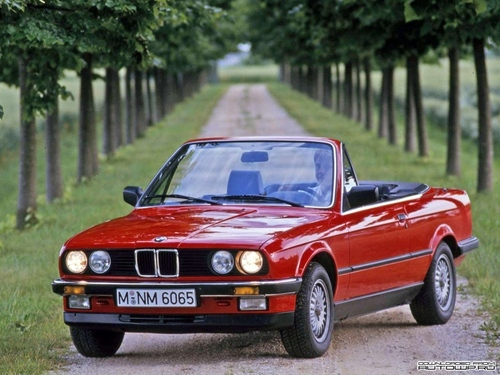
\includegraphics[width=2.5in]{bmw} \\
      \end{center} \pause

      \begin{columns}[onlytextwidth]
        \column{.5\textwidth}
          \begin{itemize}
            \item Cylinders
            \item Displacement
            \item Horsepower
          \end{itemize}
        \column{.5\textwidth}
          \begin{itemize}
            \item Weight
            \item Acceleration
            \item Year (After 1975 or not)
          \end{itemize}
      \end{columns}
    \end{frame}

    \begin{frame}[fragile]{Exploring the data}
      \fontsm
\begin{knitrout}
\definecolor{shadecolor}{rgb}{0.137, 0.137, 0.137}\begin{kframe}
\begin{alltt}
\hlkwd{head}\hlstd{(cars)}
\end{alltt}
\begin{verbatim}
  MPG Cylinders Displacement  HP Weight Acceleration After1975 Origin
1  18         8          307 130   3504         12.0        No     US
2  15         8          350 165   3693         11.5        No     US
3  18         8          318 150   3436         11.0        No     US
4  16         8          304 150   3433         12.0        No     US
5  17         8          302 140   3449         10.5        No     US
6  15         8          429 198   4341         10.0        No     US
\end{verbatim}
\end{kframe}
\end{knitrout}
      \pause
      How do we handle the Yes/No data in the \texttt{After1975} column?
    \end{frame}


    \begin{frame}[fragile]{Are late-model cars different?}
\begin{knitrout}
\definecolor{shadecolor}{rgb}{0.137, 0.137, 0.137}\begin{kframe}
\begin{alltt}
\hlkwd{boxplot}\hlstd{(MPG} \hlopt{~} \hlstd{After1975,} \hlkwc{data}\hlstd{=cars,} \hlkwc{ylab}\hlstd{=}\hlstr{"MPG"}\hlstd{,}
              \hlkwc{xlab}\hlstd{=}\hlstr{"After 1975"}\hlstd{,} \hlkwc{col}\hlstd{=}\hlstr{'darkgray'}\hlstd{)}
\end{alltt}
\end{kframe}
\input{/tmp/figures/unnamed-chunk-4-1.tex}

\end{knitrout}
    \end{frame}

    \begin{frame}[fragile]{Exploring the data}
      To incorporate the \texttt{After1975} variable into a regression model, we create a \alert{dummy variable} called \texttt{LateModel} that maps a ``Yes'' to 1, and ``No'' to 0. \pause
\begin{knitrout}
\definecolor{shadecolor}{rgb}{0.137, 0.137, 0.137}\begin{kframe}
\begin{alltt}
\hlstd{cars}\hlopt{$}\hlstd{LateModel} \hlkwb{<-}
  \hlkwd{ifelse}\hlstd{(cars}\hlopt{$}\hlstd{After1975} \hlopt{==} \hlstr{"Yes"}\hlstd{,} \hlnum{1}\hlstd{,} \hlnum{0}\hlstd{)}
\end{alltt}
\end{kframe}
\end{knitrout}
      \pause
      Now let's a regression model using the predictors \texttt{Cylinders}, \texttt{Displacement}, \texttt{HP}, \texttt{Weight}, \texttt{Acceleration}, and \texttt{LateModel}.
    \end{frame}

    \begin{frame}
      \begin{center}
        R will actually create this ``dummy'' (0/1) variable for us automatically, when you put a categorical variable (what R calls a ``factor'' into a model).
      \end{center}
    \end{frame}

    \begin{frame}[fragile]
      \fontsm
\begin{knitrout}
\definecolor{shadecolor}{rgb}{0.137, 0.137, 0.137}\begin{kframe}
\begin{alltt}
\hlkwd{summary}\hlstd{(}\hlkwd{lm}\hlstd{(MPG} \hlopt{~} \hlstd{Cylinders} \hlopt{+} \hlstd{Displacement} \hlopt{+} \hlstd{HP} \hlopt{+} \hlstd{Weight} \hlopt{+}
    \hlstd{Acceleration} \hlopt{+} \hlstd{After1975,} \hlkwc{data}\hlstd{=cars))}
\end{alltt}
\begin{verbatim}

Call:
lm(formula = MPG ~ Cylinders + Displacement + HP + Weight + Acceleration + 
    After1975, data = cars)

Residuals:
    Min      1Q  Median      3Q     Max 
-8.9302 -2.5727 -0.2574  2.0630 15.0381 

Coefficients:
               Estimate Std. Error t value Pr(>|t|)    
(Intercept)  42.1939988  2.3687735  17.813  < 2e-16 ***
Cylinders    -0.5840362  0.3601220  -1.622    0.106    
Displacement  0.0074811  0.0079791   0.938    0.349    
HP           -0.0198909  0.0147848  -1.345    0.179    
Weight       -0.0059904  0.0007194  -8.327 1.46e-15 ***
Acceleration  0.0354327  0.1103506   0.321    0.748    
After1975Yes  4.3590043  0.4016220  10.853  < 2e-16 ***
---
Signif. codes:  0 '***' 0.001 '**' 0.01 '*' 0.05 '.' 0.1 ' ' 1

Residual standard error: 3.721 on 385 degrees of freedom
Multiple R-squared:  0.7762,	Adjusted R-squared:  0.7727 
F-statistic: 222.5 on 6 and 385 DF,  p-value: < 2.2e-16
\end{verbatim}
\end{kframe}
\end{knitrout}
    \end{frame}

    \begin{frame}[fragile]{Dummy variables}
      \texttt{After1975Yes} is 1 whenever \texttt{After1975} is ``Yes,'' and 0 otherwise:

      \begin{table}[!b]
        {\carlitoTLF % Use monospaced lining figures
        \begin{tabularx}{\textwidth}{rrrrr}

           MPG &  ... & Acceleration & After1975 & After1975Yes\\
          \toprule
            ... & ... & ... & ... & ... \\
            25 & ... & 13.5 & No & 0 \\
            33 & ... & 17.5 & No & 0 \\
            28 & ... & 15.5 & Yes & 1 \\
            25 & ... & 16.9 & Yes & 1 \\
            ... & ... & ... & ... & ... \\
          \bottomrule

        \end{tabularx}}

      \end{table}

      \pause
      Notice that we do not have a \texttt{After1975No} variable; it would cause problems because it would be perfectly correlated with \texttt{After1975Yes}.
    \end{frame}

    \begin{frame}[fragile]{Interpretation of the $\hat\beta$ of the dummy variable}
      
      Our regression equation is:
      \[
        \widehat{\text{MPG}} = 41.71 -
        0.02 \cdot \text{HP} -
        0.01 \cdot \text{Weight} +
        4.33 \cdot \text{After1975Yes}.
      \]
      \pause

      Let's interpret the coefficient 4.33.
      Consider this:
      \begin{itemize}[<+->]
        \item Model A and B have the same HP and Weight.
        \item Model A was manufactured before 1975, whereas B was manufactured after 1975.
        \item We predict Model B will have a MPG that is 4.33 higher than Model A.
      \end{itemize}
      \lc
    \end{frame}

    \begin{frame}[fragile]{Interpretation of the $\hat\beta$ of the dummy variable}
      R has assigned ``Yes'' to 1 and ``No'' to 0 in our dummy variable, so the ``reference level'' is cars manufactured before 1975.
      \pause\bigskip

      If we created a dummy variable \texttt{After1975No} that is 1 for cars manufactured \emph{before} 1975, what would the regression look like?
    \end{frame}

    \begin{frame}[fragile]{What if there are more than two categories?}
      The \texttt{Origin} variable represents the country of manufacture:
\begin{knitrout}
\definecolor{shadecolor}{rgb}{0.137, 0.137, 0.137}\begin{kframe}
\begin{alltt}
\hlkwd{boxplot}\hlstd{(MPG} \hlopt{~} \hlstd{Origin,} \hlkwc{data}\hlstd{=cars,} \hlkwc{ylab}\hlstd{=}\hlstr{"MPG"}\hlstd{,}
              \hlkwc{xlab}\hlstd{=}\hlstr{"Origin"}\hlstd{,} \hlkwc{col}\hlstd{=}\hlstr{'darkgray'}\hlstd{)}
\end{alltt}
\end{kframe}
\input{/tmp/figures/unnamed-chunk-8-1.tex}

\end{knitrout}
    \end{frame}

    \begin{frame}[fragile]{What if there are more than two categories?}
      \begin{itemize}[<+->]
        \item The \texttt{Origin} variable has 3 ``levels''---US, EU, and JP---so we can't easily convert this into a 0/1 dummy variable.
        \item The solution is to create a dummy variable for \emph{each} level (category), and include \alert{all but one} of them as predictors in the model.
        \item The category left out is the \alert{reference level} and all slope coefficients for dummy variables are interpreted as the difference between that category and the reference level.
        \item If \emph{any} of the dummy variables are significant for a particular categorical variable, we consider the entire categorical variable to be significant!
      \end{itemize}
    \end{frame}

    \begin{frame}[fragile]
      \fontsm\vspace{-0.15in}
\begin{knitrout}
\definecolor{shadecolor}{rgb}{0.137, 0.137, 0.137}\begin{kframe}
\begin{alltt}
\hlstd{origin.model} \hlkwb{<-} \hlkwd{lm}\hlstd{(MPG} \hlopt{~} \hlstd{HP} \hlopt{+} \hlstd{Weight} \hlopt{+} \hlstd{After1975} \hlopt{+} \hlstd{Origin,} \hlkwc{data}\hlstd{=cars)}
\hlkwd{summary}\hlstd{(origin.model)}
\end{alltt}
\begin{verbatim}

Call:
lm(formula = MPG ~ HP + Weight + After1975 + Origin, data = cars)

Residuals:
   Min     1Q Median     3Q    Max 
-9.705 -2.243 -0.199  1.816 13.789 

Coefficients:
              Estimate Std. Error t value Pr(>|t|)    
(Intercept)  40.181974   0.874271   45.96   <2e-16 ***
HP           -0.027984   0.009865   -2.84   0.0048 ** 
Weight       -0.005160   0.000477  -10.81   <2e-16 ***
After1975Yes  4.334280   0.392849   11.03   <2e-16 ***
OriginJP      1.000586   0.611954    1.64   0.1029    
OriginUS     -1.592573   0.561900   -2.83   0.0048 ** 
---
Signif. codes:  0 '***' 0.001 '**' 0.01 '*' 0.05 '.' 0.1 ' ' 1

Residual standard error: 3.6 on 386 degrees of freedom
Multiple R-squared:  0.787,	Adjusted R-squared:  0.784 
F-statistic:  285 on 5 and 386 DF,  p-value: <2e-16
\end{verbatim}
\end{kframe}
\end{knitrout}
    \end{frame}

    \begin{frame}[fragile]{A warning about categorical variables with numeric representations}
      \begin{itemize}[<+->]
        \item In the original dataset, the origin was represented as 1 for US, 2 for EU and 3 for JP.
        \item We would \alert{not} want to just put these numbers in the regression as numbers, because then regression would treat this as if it were a quantitative variable!
        \item Even though the representation in the file is numeric, it is still a categorical variable and should be treated as such.
      \end{itemize}
    \end{frame}

    \begin{frame}[fragile]{A warning about categorical variables with numeric representations}
\begin{knitrout}
\definecolor{shadecolor}{rgb}{0.137, 0.137, 0.137}
\input{/tmp/figures/unnamed-chunk-10-1.tex}

\end{knitrout}
    \end{frame}

    \begin{frame}[fragile]{Statistical significance of a categorical variable}
      While dealing with categorical variables, we want to look at the significance of the categorical variable as a whole, rather than looking at $p$-values of individual dummy variables.

      \bigskip\pause

      We want to test the \alert{compound null hypothesis}
      \[
        H_0 : \beta_{\text{US}} = \beta_{\text{JP}} = 0.
      \]
    \end{frame}

    \begin{frame}[fragile]{Statistical significance of a categorical variable}
      To do this, we look at the ANOVA table; the $p$-value on the Origin line ($2.4 \times 10^{-5}$) is the $p$-value for the compound null hypothesis $H_0 : \beta_{\text{US}} = \beta_{\text{JP}} = 0$.
      \fontsm
\begin{knitrout}
\definecolor{shadecolor}{rgb}{0.137, 0.137, 0.137}\begin{kframe}
\begin{alltt}
\hlkwd{anova}\hlstd{(origin.model)}
\end{alltt}
\begin{verbatim}
Analysis of Variance Table

Response: MPG
           Df Sum Sq Mean Sq F value  Pr(>F)    
HP          1  14433   14433  1096.0 < 2e-16 ***
Weight      1   2392    2392   181.6 < 2e-16 ***
After1975   1   1623    1623   123.2 < 2e-16 ***
Origin      2    288     144    10.9 2.4e-05 ***
Residuals 386   5083      13                    
---
Signif. codes:  0 '***' 0.001 '**' 0.01 '*' 0.05 '.' 0.1 ' ' 1
\end{verbatim}
\end{kframe}
\end{knitrout}
    \end{frame}

    \begin{frame}{Practical significance of a categorical variable}
      
      Since $p<.05$, we can conclude that Origin is a statistically significant predictor of MPG.
      But is it a \emph{practically} significant predictor?

      \bigskip\pause

      To do this, compare $R^2$ values, or standard error of residuals:

      \bigskip

      \begin{tabular}{lll}
      \textbf{Model} & \textbf{$R^2$} & \textbf{Residual standard error} \\
      \hline
      \texttt{Origin} not included in model & 0.77 & 3.72 \\
      \texttt{Origin} included in model & 0.79 & 3.63 \\
      \hline
      \end{tabular}

      \bigskip

      We have to decide if the increased precision is worth the extra complexity in the model.
    \end{frame}
  \end{darkframes}

\end{document}
